\subsection{המטען האפקטיבי}
בדומה לאטום ההליום, בסביבת הגרעין המטען האפקטיבי הוא בקירוב מטען הגרעין, ורחוק מהגרעין, המטען האפקטיבי הוא מתכנס להיות בערך $-1$.

\begin{figure}[h!]
    \centering
    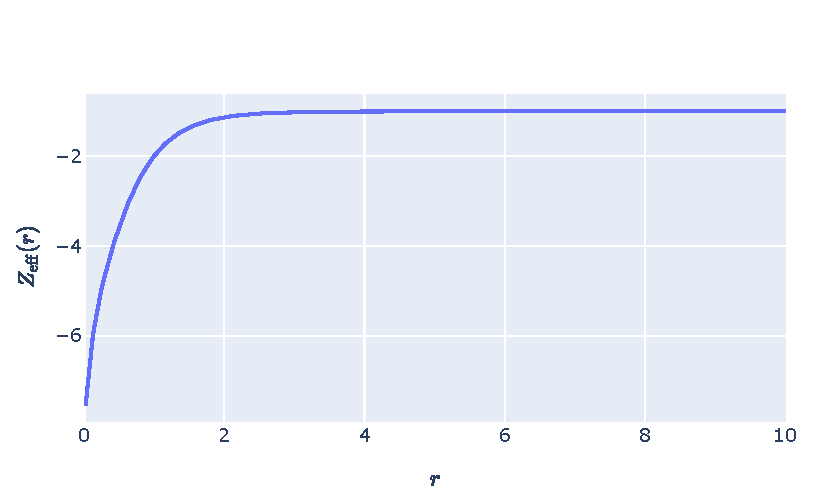
\includegraphics[width=0.5\linewidth]{plots/oxygen_atom/effective_charge.eps}
    \caption{המטען האפקטיבי באיטרציה האחרונה}
    \label{fig:O_effective_charge}
\end{figure}
